\documentclass[a4paper,10pt]{article}
\usepackage[dvips]{color,graphicx}
\usepackage[dvips, bookmarks, colorlinks=false]{hyperref}


%opening
\title{Math508 Homework 11}
\author{Yu Huang}

\begin{document}

\maketitle

\begin{abstract}
Simulation of a frequency filtering
\end{abstract}

\section{Problem 3}
\begin{equation}
Re(\theta_n) = \eta_1 cos(\lambda_1 n)
\end{equation}

\begin{equation}
Re(X_n) = \eta_1 cos(\lambda_1 n) + \eta_2 cos(\lambda_2 n)
\end{equation}

\begin{equation}
Re(Y_n^M) = (1-a^2)((M+1)\eta_1 cos(\lambda_1 n) + \sum_{k=0}^M \eta_2 cos(\lambda_2 n + (\lambda_1-\lambda_2) k))
\end{equation}

Figure~\ref{f1} is plot of the real parts of $\theta_n$ and $X_n$. Figure~\ref{f2} is plot of the real parts of $\theta_n$ and $Y_n^M$.

\begin{figure}
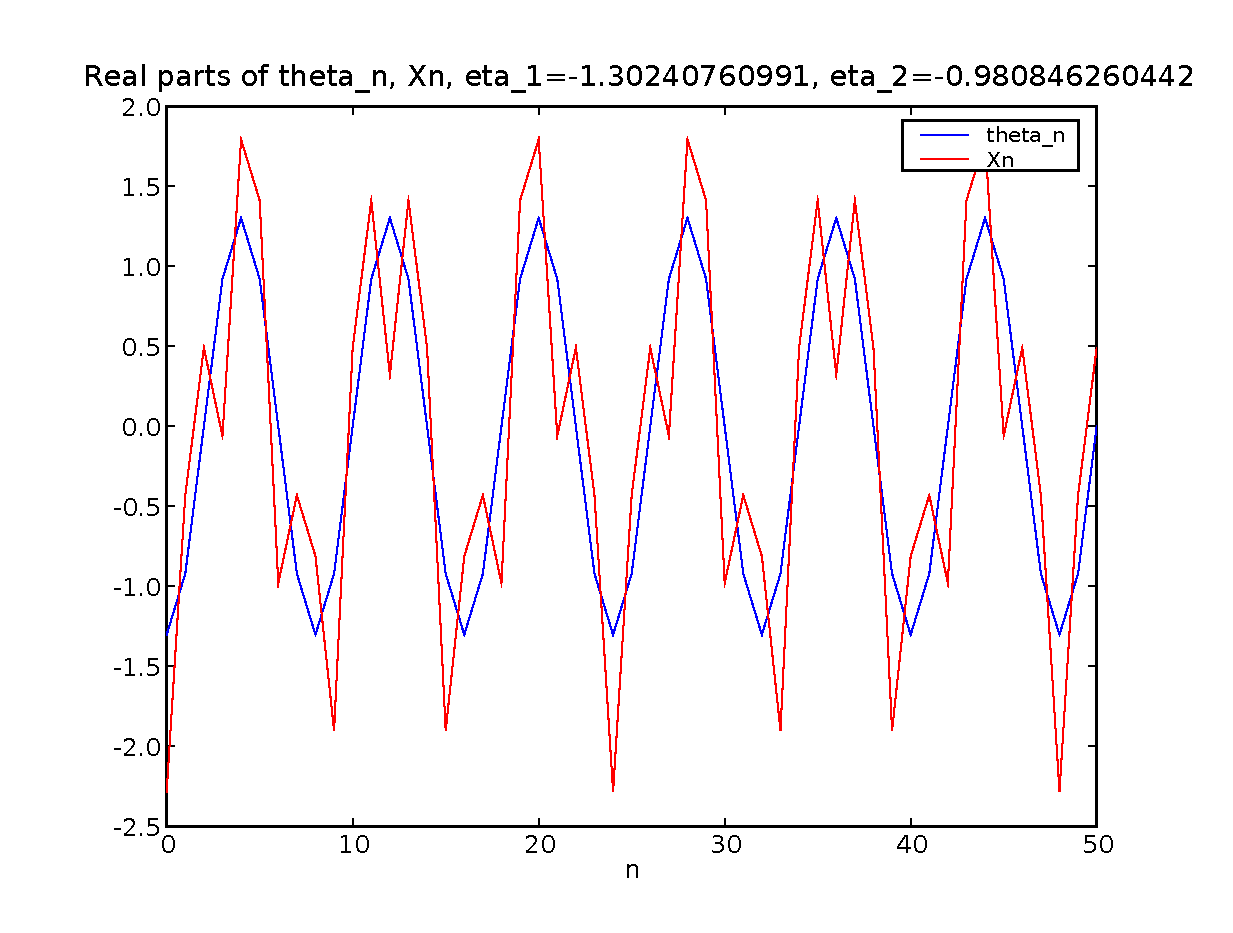
\includegraphics[width=1\textwidth]{hw11_3_theta_n_Xn.eps}
\caption{}\label{f1}
\end{figure}

\begin{figure}
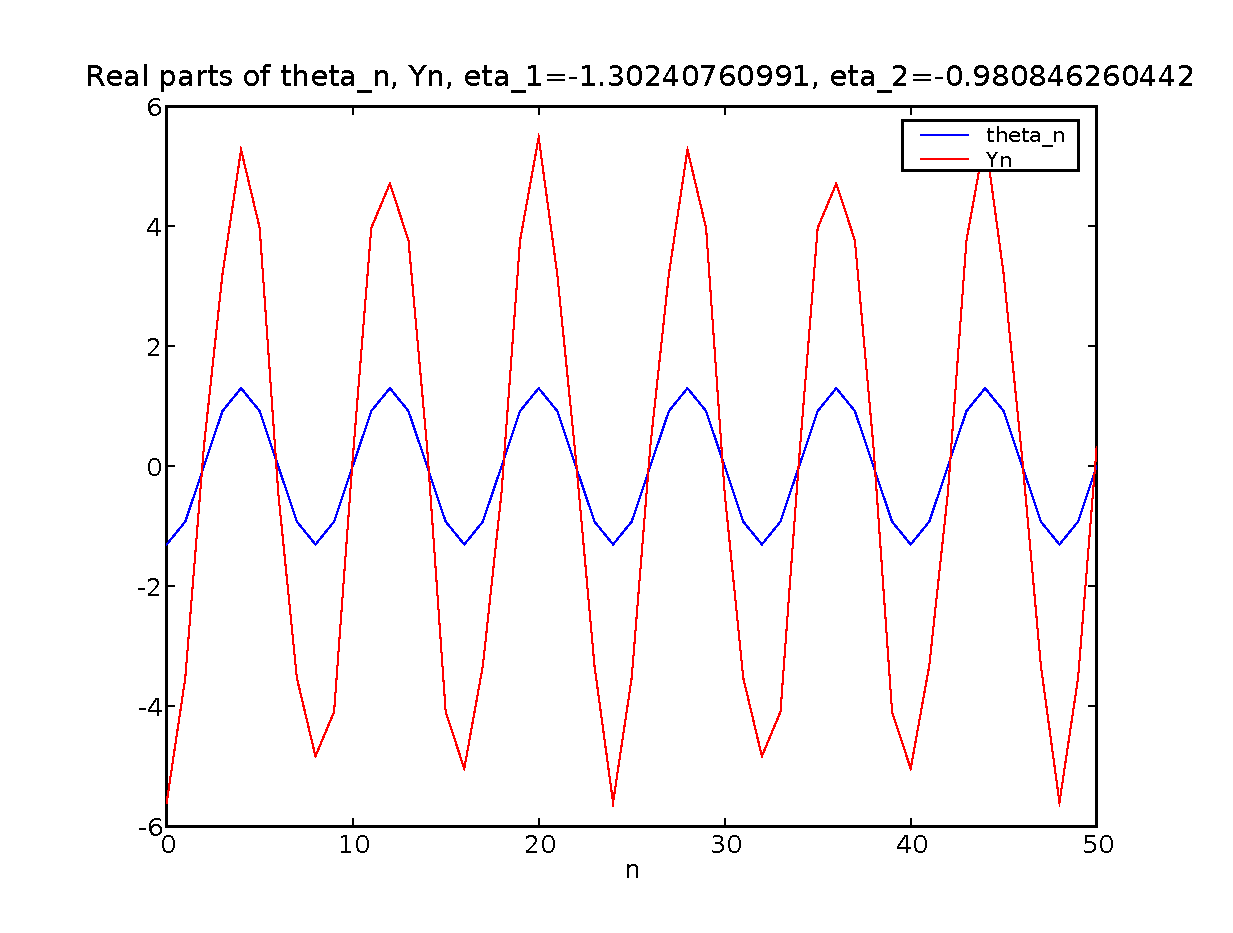
\includegraphics[width=1\textwidth]{hw11_3_theta_n_Yn.eps}
\caption{}\label{f2}
\end{figure}



\end{document}
